%%%%%%%%%%%%%%%%%%%%%%%%%%%%%%%%%%%%%%%%%%%%%%%%
\section{Final example}


%%%%%%%%%%%%%%%%%%%%%%%%%%%%%%%%%%%%%%%%%%%%%%%%%%%%%%%
\begin{frame}

\frametitle{Graph}

\begin{figure}
  \centering
  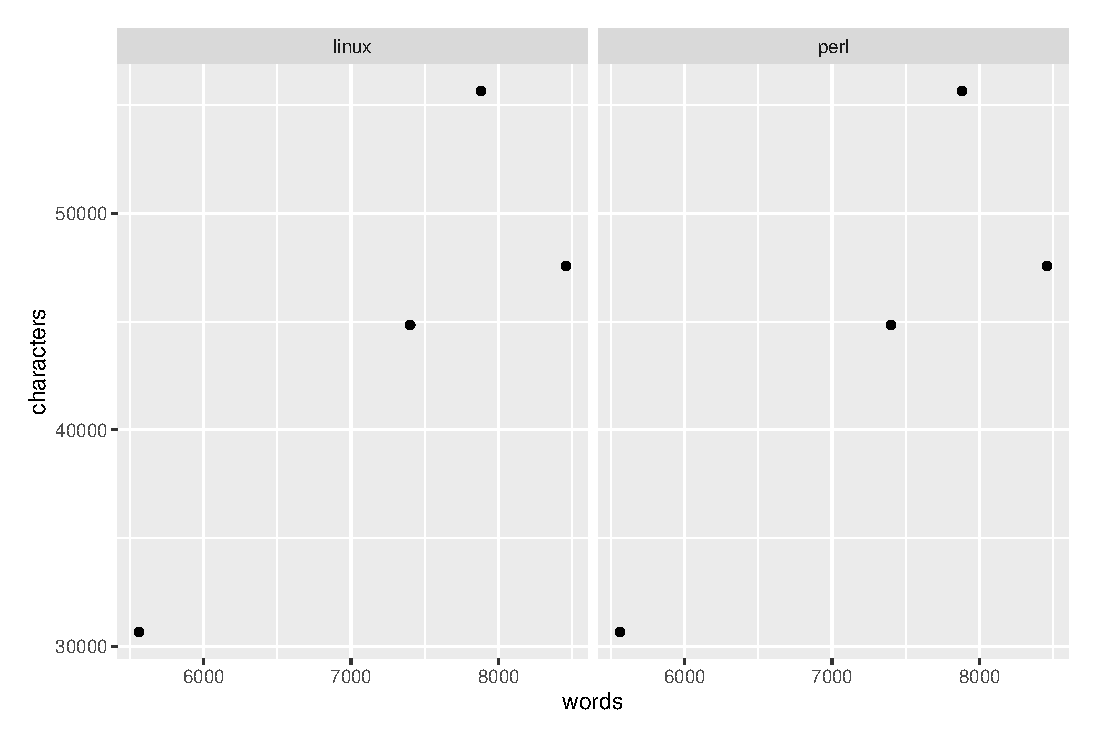
\includegraphics[width=10cm]{finalex/canterbury}
\end{figure}

\end{frame}


%%%%%%%%%%%%%%%%%%%%%%%%%%%%%%%%%%%%%%%%%%%%%%%%%%%%%%%
\begin{frame}

\frametitle{Data table}

Create a data table in tab-separated format:  {\texttt{fileslist.tsv}}.

\begin{table}
  \begin{tabular}{ccc}
  \hline
ID & corpus & filename \\
  \hline
1 & calgary & book1 \\
2 & calgary & book2 \\
3 & calgary & news \\
4 & calgary & progc \\
5 & calgary & progl \\
6 & calgary & progp \\
7 & canterbury & alice29 \\
8 & canterbury & asyoulik \\
9 & canterbury & lcet10 \\
10 & canterbury & plrabn12 \\
  \hline
  \end{tabular}
\end{table}

\end{frame}


%%%%%%%%%%%%%%%%%%%%%%%%%%%%%%%%%%%%%%%%%%%%%%%%%%%%%%%
\begin{frame}[fragile]

\frametitle{Main Snakefile\footnote{V6}}

\begin{tiny}
\begin{lstlisting}[frame=single,language=bash]
import pandas as pd

from snakemake.utils import validate, min_version

configfile: "config.yml"
validate (config, schema = "config.schema.yml")

fileslist_panda = pd.read_table (config["fileslist"], sep='\t', lineterminator='\n')
fileslist_panda.set_index ("ID", drop=False, inplace=True)
validate (fileslist_panda, schema="fileslist.schema.yml")

##  Define global constraints on wildcards
wildcard_constraints:
  corpus = "calgary|canterbury"

##  Include important variables
include:  "global-vars.smk"

include:  "single.smk"
include:  "combine.smk"
include:  "graphs.smk"

rule all:
  input:
    OUTPUT_DIR + "/05-graphs/canterbury.jpg"
\end{lstlisting}
\end{tiny}

\end{frame}


%%%%%%%%%%%%%%%%%%%%%%%%%%%%%%%%%%%%%%%%%%%%%%%%%%%%%%%
\begin{frame}[fragile]

\frametitle{{\texttt{graphs.smk}}\footnote{V6}}

\begin{tiny}
\begin{lstlisting}[frame=single,language=bash]
rule Scatterplot:
  input:
    input_fn1 = OUTPUT_DIR + "/04-combine-perl/{corpus}.tsv",
    input_fn2 = OUTPUT_DIR + "/04-combine-linux/{corpus}.tsv",
  output:
    output_fn1 = OUTPUT_DIR + "/05-graphs/{corpus}.jpg",
    output_fn2 = OUTPUT_DIR + "/05-graphs/{corpus}.png",
    output_fn3 = OUTPUT_DIR + "/05-graphs/{corpus}.eps"
  params:
    corpus = "{corpus}",
    myeps = lambda wildcards: config["my_options"]["postscript"]
  log:
    log_fn1 = OUTPUT_DIR + "/05-graphs/{corpus}.log"
  shell:
    """
    ##  {params.corpus} is available
    mypng="png"
    {TOOLS_DIR}/scatterplot.R --type jpg --perl {input.input_fn1} --linux
      {input.input_fn2} --output {output.output_fn1} >{log.log_fn1} 2>&1
    {TOOLS_DIR}/scatterplot.R --type ${{mypng}} --perl {input.input_fn1} --linux
      {input.input_fn2} --output {output.output_fn2} >>{log.log_fn1} 2>&1
    {TOOLS_DIR}/scatterplot.R --type {params.myeps} --perl {input.input_fn1} --linux
      {input.input_fn2} --output {output.output_fn3} >>{log.log_fn1} 2>&1
    """
\end{lstlisting}
\end{tiny}

\end{frame}


%%%%%%%%%%%%%%%%%%%%%%%%%%%%%%%%%%%%%%%%%%%%%%%%%%%%%%%
\begin{frame}[fragile]

\frametitle{{\texttt{combine.smk}}\footnote{V6}}

\begin{tiny}
\begin{lstlisting}[frame=single,language=bash]
rule CombinePerl:
  input:  GatherPerl
  output:  OUTPUT_DIR + "/04-combine-perl/{corpus}.tsv"
  shell:
    """
    cat {input} >{output}
    """
\end{lstlisting}
\end{tiny}

\end{frame}


%%%%%%%%%%%%%%%%%%%%%%%%%%%%%%%%%%%%%%%%%%%%%%%%%%%%%%%
\begin{frame}[fragile]

\frametitle{{\texttt{combine.smk}}\footnote{V6}}

\begin{tiny}
\begin{lstlisting}[frame=single,language=python]
def GatherPerl (wc):
  results = []  ##  Initialise empty list

  ##  Iterate through each row of the table
  for row in fileslist_panda.itertuples (index = False):
    curr_ID = str (row.ID)  ##  Convert integer to string
    curr_corpus = row.corpus  ##  Current "corpus" in this row
    curr_filename = row.filename

    ##  Check for equality between wildcard corpus and current corpus
    if wc.corpus == curr_corpus:
      d = [OUTPUT_DIR + "/02-count-perl/{f}.count".format (f=curr_filename)]
      results.extend (d)  ##  Add it to the list

  ##  Print out the results
  print (results, file=sys.stderr)

  return results
\end{lstlisting}
\end{tiny}
\pause

The {\texttt{print ()}} produces this:
\begin{tiny}
\begin{lstlisting}[frame=single,language=bash]
['Output/02-count-perl/alice29.count', 'Output/02-count-perl/asyoulik.count',
'Output/02-count-perl/lcet10.count', 'Output/02-count-perl/plrabn12.count']
\end{lstlisting}
\end{tiny}

\end{frame}


%%%%%%%%%%%%%%%%%%%%%%%%%%%%%%%%%%%%%%%%%%%%%%%%%%%%%%%
\begin{frame}[fragile]

\frametitle{Visualisation\footnote{V6}}

\begin{figure}
  \centering
  {\fbox{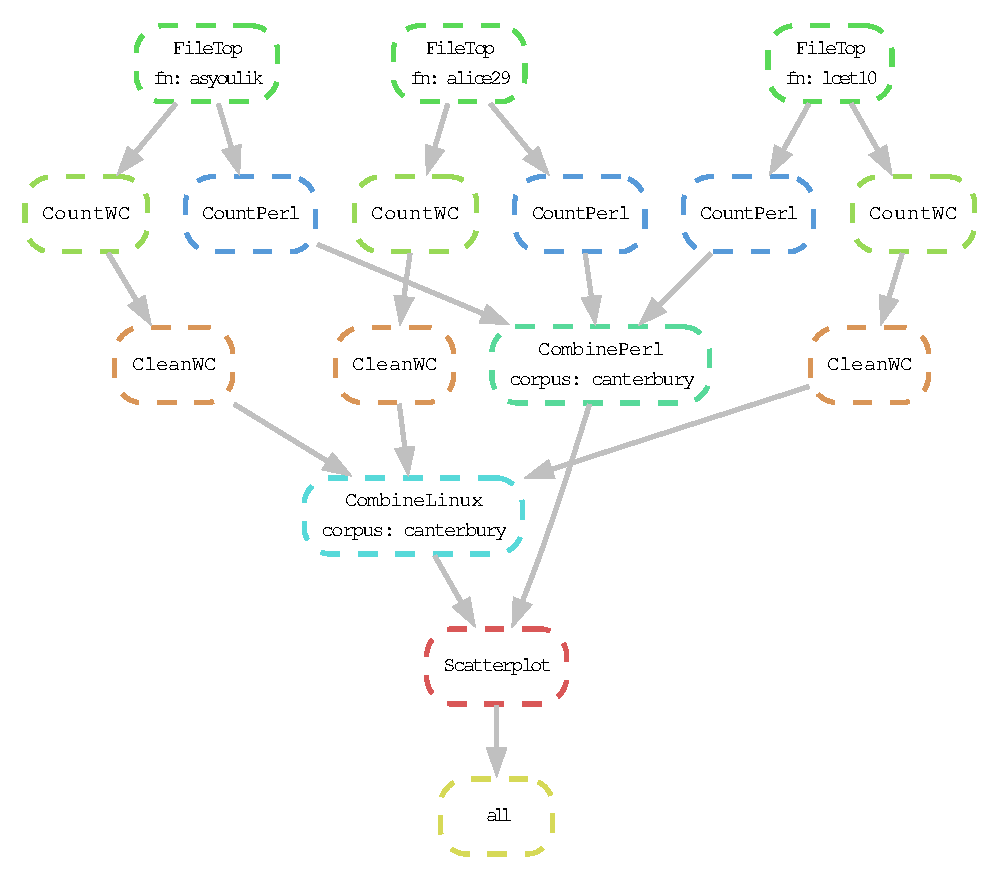
\includegraphics[width=9cm]{finalex/dag-v6}}}
\end{figure}

\end{frame}


%%%%%%%%%%%%%%%%%%%%%%%%%%%%%%%%%%%%%%%%%%%%%%%%%%%%%%%
\begin{frame}[fragile]

\frametitle{Update the all rule}

This can also be done to the {\magenta{all}} rule to process both corpora:
\begin{tiny}
\begin{lstlisting}[frame=single,language=bash]
rule all:
  input:
    OUTPUT_DIR + "/05-graphs/canterbury.jpg",
    OUTPUT_DIR + "/05-graphs/calgary.jpg"
\end{lstlisting}
\end{tiny}

\end{frame}


%%%%%%%%%%%%%%%%%%%%%%%%%%%%%%%%%%%%%%%%%%%%%%%%%%%%%%%
\begin{frame}[fragile]

\frametitle{Some things to note}

\begin{tiny}
\begin{lstlisting}[frame=single,language=bash]
rule Scatterplot:
  input:
    input_fn1 = OUTPUT_DIR + "/04-combine-perl/{corpus}.tsv",
    input_fn2 = OUTPUT_DIR + "/04-combine-linux/{corpus}.tsv",
  output:
    output_fn1 = OUTPUT_DIR + "/05-graphs/{corpus}.jpg",
    output_fn2 = OUTPUT_DIR + "/05-graphs/{corpus}.png",
    output_fn3 = OUTPUT_DIR + "/05-graphs/{corpus}.eps"
  params:
    corpus = "{corpus}",
    myeps = lambda wildcards: config["my_options"]["postscript"]
  log:
    log_fn1 = OUTPUT_DIR + "/05-graphs/{corpus}.log"
  shell:
    """
    ##  {params.corpus} is available
    mypng="png"
    {TOOLS_DIR}/scatterplot.R --type jpg --perl {input.input_fn1} --linux
      {input.input_fn2} --output {output.output_fn1} >{log.log_fn1} 2>&1
    {TOOLS_DIR}/scatterplot.R --type ${{mypng}} --perl {input.input_fn1} --linux
      {input.input_fn2} --output {output.output_fn2} >>{log.log_fn1} 2>&1
    {TOOLS_DIR}/scatterplot.R --type {params.myeps} --perl {input.input_fn1} --linux
      {input.input_fn2} --output {output.output_fn3} >>{log.log_fn1} 2>&1
    """
\end{lstlisting}
\end{tiny}

\end{frame}


%%%%%%%%%%%%%%%%%%%%%%%%%%%%%%%%%%%%%%%%%%%%%%%%%%%%%%%
\begin{frame}

\frametitle{Some things to note}

\begin{itemize}
  \item R script is meant to run on the command-line with supplied arguments (i.e., not interactively in RStudio).
  \item There is a {\blue{log file}}!  If a rule fails, Snakemake deletes all output generated (i.e., in the output directive).  Those sent to the log directive are {\red{not}}.  Looking at them will save you many headaches.
  \item I have given {\green{names}} to the input, output, and log directives.  Without names and as a list, you can also refer to files with an index:  {\texttt{input[2]}} (i.e., the third file in the input directive)
\end{itemize}

\end{frame}


%%%%%%%%%%%%%%%%%%%%%%%%%%%%%%%%%%%%%%%%%%%%%%%%%%%%%%%
\begin{frame}[fragile]

\frametitle{Some things to note}

From {\texttt{config.yml}}:
\begin{tiny}
\begin{lstlisting}[frame=single,language=bash]
fileslist:  "fileslist.tsv"

my_options:
  postscript:  "eps"
\end{lstlisting}
\end{tiny}

\begin{itemize}
  \item Note 3 ways the argument to {\texttt{--type}} is provided and used:
  \begin{enumerate}
    \item {\texttt{jpg}} as literal text
    \item {\texttt{png}} as a bash variable
    \item {\texttt{eps}} as a Snakemake variable which is stored in a file called {\texttt{config.yml}}.  Note the use of {\texttt{lambda}} to access the dictionary created by the configuration file.
  \end{enumerate}
\end{itemize}

\end{frame}


%%%%%%%%%%%%%%%%%%%%%%%%%%%%%%%%%%%%%%%%%%%%%%%%%%%%%%%
\begin{frame}

\frametitle{Much larger Snakemake example}

\begin{figure}
  \centering
  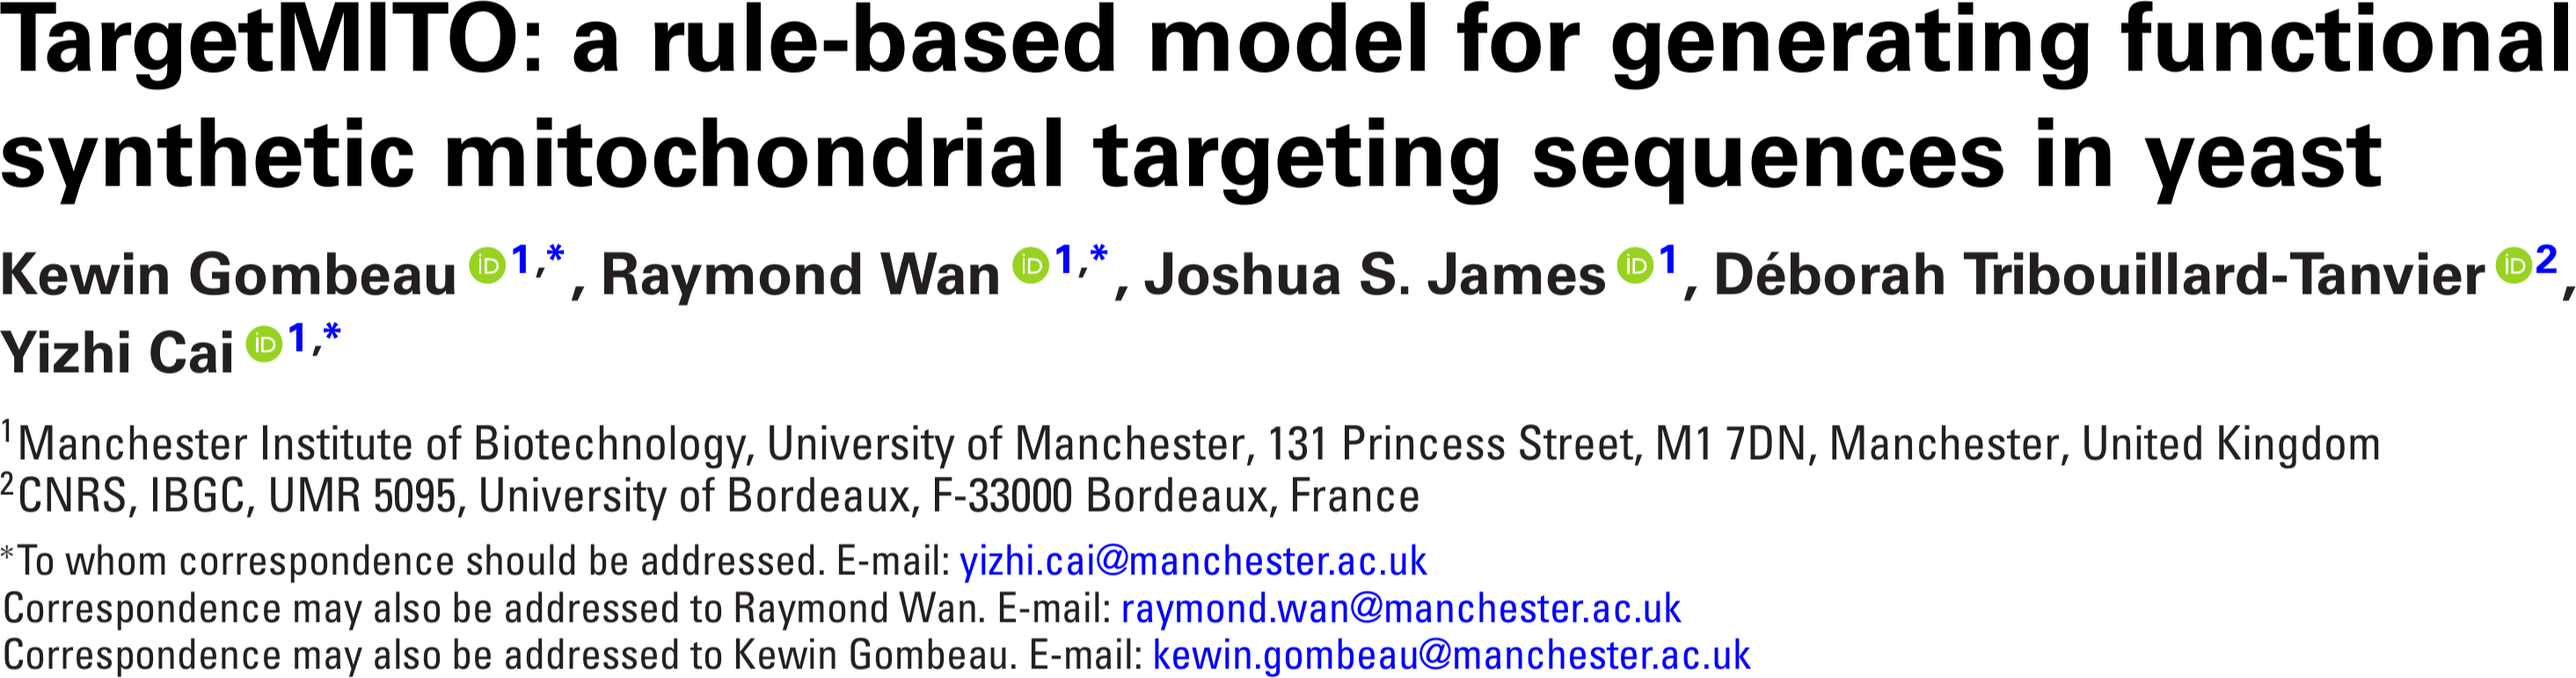
\includegraphics[width=\linewidth]{structure/gwjtc26-nar}
\end{figure}

\end{frame}


%%%%%%%%%%%%%%%%%%%%%%%%%%%%%%%%%%%%%%%%%%%%%%%%%%%%%%%
\begin{frame}

\frametitle{Larger Snakemake example}

GitHub repository (\href{https://github.com/the-cai-lab/synMTS}{https://github.com/the-cai-lab/synMTS}) has 4 workflows meant to run in order:

\begin{enumerate}
  \item generate -- Generate synthetic mitochondria targeting sequences (synMTS)
  \item evaluate -- Evaluate these sequences
  \item statistics -- Calculate some statistics over the properties of the synMTS
  \item select -- Take a subset of the results to focus on [for the manuscript]
\end{enumerate}

\end{frame}


